In BGV, BFV and CKKS the ciphertext modulus $Q$ is large --- much larger than a computer word (typically 64 bits on modern computers). Multi-precision arithmetic is known to be slow due to its serial nature, so implementations avoid it by using a \gls{rns}, which represents large numbers as a set of smaller, independent residues. RNS variants of BGV, BFV and CKKS are the standard in practice; OpenFHE, for example, only supports the RNS versions of these schemes.

\begin{definition}[Canonical Form]
    We are interested in polynomials in the ring $R_Q = \mathbb{Z}_Q[X]/(X^N+1)$ with degree (up to) $N - 1$ and coefficients in $[-Q/2, Q/2)$ (centered modulo representation), and different ways to represent this polynomial. The canonical form \eqref{form:canonical} of such a polynomial $a$ is the form everyone is familiar with.
    \begin{equation}
        \label{form:canonical}
        a = c_0 + c_1X + \cdots + c_{N-1}X^{N-1} = \sum_{i=0}^{N-1} c_iX^i
    \end{equation}
\end{definition}

\begin{definition}[Coefficient Form]
    As polynomials have a well-known/predictable structure, we can omit the redundant $X$ variable and represent $a\in R_Q$ uniquely by its coefficients. I will refer to (only) this representation \eqref{form:coefficient} as the \emph{coefficient} form.  
    \begin{equation}
        \label{form:coefficient}
        a = (c_0, c_1, \dots, c_{N-1})
    \end{equation}
\end{definition}

Let $Q = q_0\dots q_{k-1}$ with $\gcd(q_i, q_j) = 1 \;\forall\; i\not= j$, so that the \gls{crt} allows decomposition into smaller residues. If $\max_i\{q_i\}$ fits in a computer word then we can use \gls{crt} on the coefficients of a polynomial to work exclusively with integers that fit inside a computer word.

%%
%% COEFFICIENT FORMAT
\begin{definition}[CRT Form]
    Given a polynomial $a \in R_Q$ where $Q = q_0q_1\dots q_{k-1}$ is chosen as a product of $k$ small primes (small meaning they each fit inside a computer register), each coefficient $c_i$ is uniquely represented by its $k$ residues via the Chinese Remainder Theorem. Then the \emph{CRT form} of $a$ \eqref{form:crt} is a collection of smaller polynomials ($\bmod{q_i}$) called \textit{towers}, \textit{residues} or \textit{limbs}.

    \begin{equation}
    \label{form:crt}
    % \ifnotes
        \begin{pmatrix}
            a\mod q_0 \\
            a\mod q_1 \\
            \vdots \\
            a\mod q_{k-1}
        \end{pmatrix}
        =
    % \fi
    \begin{pmatrix}
        c_0 \bmod{q_0} & c_1 \bmod{q_0} & \dots & c_{N-1}\bmod{q_0} \\
        c_0 \bmod{q_1} & c_1 \bmod{q_1} & \dots & c_{N-1}\bmod{q_1} \\
        \vdots & \vdots & \ddots & \vdots \\
        c_0 \bmod{q_{k-1}} & c_1 \bmod{q_{k-1}} & \dots & c_{N-1}\bmod{q_{k-1}}
    \end{pmatrix}
    \end{equation}
\end{definition}

Addition and subtraction of two polynomials in $R_Q$ is equivalent to element-wise addition/subtraction of their CRT forms (modulo $q_i$). As each element fits within a computer word, no carries propagate between them, and all pairs of elements can be added or subtracted in parallel.

% \noindent Clearly, the $i$-th column of \eqref{form:crt} is a CRT problem for $c_i$, so converting between this and the canonical form $\sum_{i=0}^{N-1}c_iX^i$ or vector form $(c_0,c_1,\dots, c_{N-1})$ is easy. \textcolor{red}{\textbf{Note that confusingly ``coefficient format'' is used in OpenFHE about this form specifically, NOT the ``vector'' form which is normally used in the literature... kjært barn har mange navn..}}

\begin{remark}
    \textcolor{red}{Rather confusingly, OpenFHE calls this form \emph{Coefficient} format. Both RNS forms are represented by an \texttt{DCRTPoly} object, so a polynomial in CRT form is represented by a \texttt{DCRTPoly} object in \texttt{Format::Coefficient} mode.}
    \begin{figure}[ht!]
        \centering
        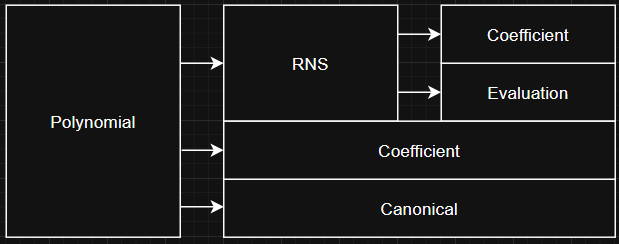
\includegraphics[width=0.4\linewidth]{Figures/representations.png}
    \end{figure}
\end{remark}

%%
%% EVALUATION FORMAT
\subsection{Number Theoretic Transform}
% Maybe more details in appendix?
The \gls{ntt} converts a negacyclic convolution in the coefficient domain into point-wise multiplication in the NTT domain --- and multiplication in $R_{q_i}$ is exactly such a convolution of the coefficient vectors. Applying the \gls{ntt} to each residue (row) of the CRT form \eqref{form:crt} therefore makes polynomial multiplication element-wise as well. The negacyclic \gls{ntt} of size $N$ requires each modulus to satisfy $q_i \equiv 1 \pmod{2N}$, which constrains the choice of RNS primes.

\begin{definition}[Double CRT/NTT/Evaluation Form]
    By applying the \gls{ntt} to the CRT form \eqref{form:crt} we gain the ability to perform polynomial multiplication in parallel, without losing the ability to perform addition/subtraction in parallel.
    
    \begin{equation}
        \label{form:eval}
        \begin{pmatrix}
            \ntt{a\bmod q_0} \\
            \ntt{a\bmod q_1} \\
            \vdots \\
            \ntt{a\bmod q_{k-1}}
        \end{pmatrix}
        =
        \begin{pmatrix}
            \hat{a}_{0,0} & \hat{a}_{0,1} & \dots & \hat{a}_{0,N-1} \\
            \hat{a}_{1,0} & \hat{a}_{1,1} & \dots & \hat{a}_{1,N-1} \\
            \vdots & \vdots & \ddots & \vdots \\
            \hat{a}_{k-1,0} & \hat{a}_{k-1,1} & \dots & \hat{a}_{k-1,N-1}
        \end{pmatrix}
    \end{equation}
    
\end{definition}

%%
%% CLOSING REMARKS
The evaluation form \eqref{form:eval} is the preferred form, as it supports parallel addition, subtraction and multiplication, but it still does not natively support \textit{all} necessary operations. Because switching between canonical/vector, CRT and NTT mode is relatively expensive --- requiring (inverse) CRTs and NTTs --- much of the relevant literature \cite{cryptoeprint:2012/099, cryptoeprint:2016/510, cryptoeprint:2018/117, cryptoeprint:2021/204} improves upon existing functions by finding new approaches and approximations that limit the number of format-switches required. 
\begin{equation*}
    \raisebox{0.3ex}{\text{ Coefficient }}
    \overset{\text{\tiny CRT}}{\underset{\text{\tiny iCRT}}{\overset{\longrightarrow}{\longleftarrow}}}
    \raisebox{0.3ex}{\text{ CRT }}
    \overset{\text{\tiny NTT}}{\underset{\text{\tiny iNTT}}{\overset{\longrightarrow}{\longleftarrow}}}
    \raisebox{0.3ex}{\text{ Evaluation (DCRT) }}
\end{equation*}

% Switching between formats is expensive so we try to stay in evaluation mode for as long as possible, only switching to coefficient/CRT form when absolutely required.